%!TEX root = ../dissertation.tex

\chapter{La presente ricerca}
\label{chap:ricerca}

\section{Studio esplorativo}
La presente ricerca nasce da una riflessione avvenuta all'interno del corso di "Psicologia della politica" delle professoresse Carraro e Lenzi all’Università di Padova. Durante il semestre è stato condotto un progetto di gruppo denominato "Hates gonna hate..?" che ha visto la collaborazione di 8 student* (Ilaria Atella, Flavia Calabrese, Enrico della Volpe, Lorenzo Manconi, Giuseppe Mignemi, Salvatore Romano, Marianna Testa, Lavinia Tredici) e una tutor (Dalila Cataldo). Questo progetto, che ha svolto funzione di studio preliminare rispetto alla presente ricerca, si poneva l'obiettivo di esplorare gli effetti delle campagne negative nel contesto online. In quell'occasione sono stati presi in considerazione i due leader politici di Lega e Movimento 5 Stelle in corsa per le elezioni politiche del 2018 (il progetto è stato svolto poco prima delle elezioni europee del maggio 2019). Sia per Di Maio che per Salvini sono quindi stati selezionati 5 post sullo stesso tema (le banche) e con un numero di interazioni paragonabile. I post pubblicati su Facebook sono stati selezionati in base a 5 categorie: un post "neutro", uno di campagna "positiva", uno di campagna "comparativa" e due di campagna "negativa", di cui uno che aveva come  target un gruppo e un'altro che aveva come  target una singola persona.

Sono stati poi collezionati 100 commenti in modo casuale dai primi 500 pubblicati in risposta ai post considerati, e sono stati ulteriormente codificati nelle categorie di "odio concorde" o "non concorde" con la posizione del politico quando venivano riscontrati insulti, parolacce o linguaggio scurrile; "positivo concorde" o "non concorde" quando invece il tono era civile, anche se non in accordo con la posizione espressa nel post; "altro" nel caso in cui il contenuto non era interpretabile o usciva dalla discussione iniziata nel post.

Tutti i contenuti sono stati categorizzati da due divers* valutat*, con un'omogeneità dei giudizi del 92\%, in caso disaccordo i post e i commenti sono stati rivalutati da tutto il gruppo, arrivando ad ottenere un campione finale di mille contenuti codificati (100 commenti per i 5 post dei 2 politici).

Benché il campione fosse ridotto, si era riscontrata una significativa relazione tra il tipo di campagna politica e il livello di odio nei commenti $\chi^{2}$ (16, N = 1027) = 204.625, p = 0.000, evidente anche dal grafico realizzato in quell'occasione [Fig. \ref{fig:primotest}], in cui si può vedere come in post negativi si arrivi addirittura a oltre il 50\% di commenti di odio.
\begin{figure}
	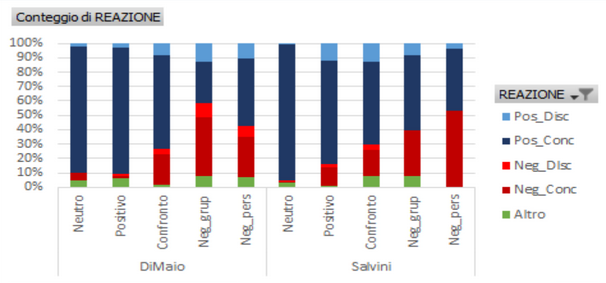
\includegraphics[width=\textwidth]{figures/primotest}
	\caption{Risultati relativi allo studio preliminare svolto durante il corso di "Psicologia della politica". Vengono messi in relazione il tipo di campanga politica contenuta nei post e i livello di odio presente nei commenti.}
	\label{fig:primotest}
\end{figure}

\section{Le nuove direzioni di sviluppo della ricerca}
Poco dopo questo studio iniziale, è stato pubblicato lo studio di Amnesty International "Barometro dell'odio", come vedremo meglio nel capitolo \nameref{chap:metodologia}. La ricerca presenta la peculiarità di raccogliere contemporaneamente i post e tweet dei politici durante la campagna elettorale, ma anche i relativi commenti, giungendo a un campione di dimensioni considerevoli. Si è deciso quindi di aggiungere al data base della ONG anche una codifica relativa al tipo di campagna utilizzata dai politici così da poter indagare, con un campione ben più esteso, il rapporto tra tipologia di campagna realizzata dai politici e generazione di odio online.
Per quanto non sia possibile determinare un principio di causalità diretto tra il tipo di campagna e il tipo di commento di odio che ne scaturisce, poiché la nostra ricerca non si avvale di un modello sperimentale, sicuramente i post dei politici precedono temporalmente le risposte delle/gli utent* e, quindi, sicuramente le influenzano.

Alla domanda relativa alla relazione tra tipo di campagna e odio nei commenti, ne sono state aggiunte alcune  suggerite dalla  letteratura del \textit{negative campaign}, e altre che indagano il  medium utilizzato, posto che il campione prende in considerazione sia Facebook che Twitter.

Per quanto riguarda l’analisi dei social , alcuni politici utilizzano in modo intercambiabile le due piattaforme analizzate in questo studio. In questi casi viene pensato a priori un contenuto o un messaggio da condividere con la propria base e lo si traduce rispettivamente in un post o un tweet che viene poi pubblicato. Altri politici invece, cambiano il linguaggio e anche i contenuti tra un piattaforma e l'altra. Abbiamo, quindi,  ritenuto interessante verificare se  il tipo di comunicazione utilizzata dai politici dipenda anche dal medium che decidono di usare se ci sono delle differenze tra l'utilizzo di \textit{negative campaign} tra le due piattaforme. Molti studi hanno dimostrato come i media tradizionali sovraespongano i messaggi di campagna negativa rispetto agli altri tipi di comunicazione \citep{walter2010} \citep{hansen2008} \citep{haselmayer2019}. Anche in relazione ai social networks, è stato evidenziato come la negatività sia più facilmente apprezzata tramite \textit{likes}, condivisioni e discussioni nei commenti \citep{conover2011} \citep{berger2010} \citep{stieglitz2013}. 

La  principale differenza tra Facebook e Twitter è sicuramente la lunghezza massima del testo che è possibile condividere: se su Facebook post lunghi e articolati sono più frequenti, su Twitter la lunghezza massima del testo è definita a priori ad un massimo di 280 caratteri.Un'altra differenza è la possibilità di interagire con gli/le utenti: se su Facebook un commento di risposta del politico potrebbe perdersi nella miriade di commenti conseguenti al post, su Twitter, tramite re-tweet e trend, è possibile instaurare vere e proprie discussioni tra politici e utenti comuni.Inoltre, Twitter è comunemente utilizzato per messaggi estemporanei di comunicazione rapida e di commento su fatti che stanno avvenendo in un momento specifico, come avviene spesso nella comunicazione politica, mentre Facebook è più utilizzato per ragionamenti complessi ed estemporanei. Analizzando le statistiche dei post e dei tweet considerati in questo studio, abbiamo cercato indicazioni anche sul diverso uso dei due social network fatto dai politici.

\section{Le ipotesi}
Le ipotesi di partenza di questa ricerca possono quindi essere suddivise in due gruppi: quelle relative alla teoria del \textit{negative campaign} (paragrafo 5.2), testate sul database dei soli post dei politici, e quelle relative alle conseguenti reazioni di odio (paragrafo 5.3) testate sui commenti in risposta ai post.
\vspace{8pt}\

Per quanto riguarda la comunicazione politica, abbiamo cercato  conferme di alcune teorie riguardo il \textit{negative campaign} presenti nella letteratura e già introdotte nel primo capitolo:

Ip.1) Il \textit{negative campaign} è in aumento rispetto ai dati registrati in altre campagne elettorali? Si vuole verificare l'ipotesi che questo tipo di campagna sia in aumento negli ultimi anni e che sia decisamente più presente rispetto a 20-30 anni fa. Verranno quindi confrontati i dati presenti in letteratura con quelli rilevati in questa ricerca, partendo dal presupposto che risulta difficile fare comparazioni tra studi che prendono in considerazioni definizioni diverse del fenomeno, analizzano mezzi di comunicazione differenti e spesso non riguardano la stessa nazione.

Ip.2) Il \textit{negative campaign} è un fenomeno diffuso prevalentemente all'interno di alcuni schieramenti politici (destra o sinistra), oppure dipende dalla posizione dei vari partiti nei luoghi del potere (governo o opposizione)? Si vuole testare l'ipotesi che questo stile comunicativo derivi dal ruolo istituzionale che gli schieramenti occupano durante la campagna e dalla conseguente strategia elettorale che ne deriva (campagna di conquista o di posizione), più che dall'orientamento politico in sé. Verranno confrontati quindi i livelli di negatività di due schieramenti diversi per orientamento politico con quelli di due schieramenti diversi per posizione istituzionale ricoperta al momento della campagna politica.

Ip.3) Il tipo di campagna politica utilizzato dipende dalla piattaforma che viene utilizzata dai politici per comunicare? In particolare è possibile rintracciare una relazione tra la brevità dei messaggi formulati su Twitter rispetto ai post mediamente più lunghi di Facebook? L'ipotesi è che il tipo di campagna utilizzato derivi dalla strategia politica che quindi dovrebbe risultare indipendente dal medium utilizzato e dal suo stile comunicativo. Verranno confrontati i livelli di negatività del discorso politico  suddividendo i post in base al sito di pubblicazione del contenuto (Twitter o Facebook).

Ip.4) I post di \textit{negative campaign} sono in media più virali rispetto a quelli positivi? Si vuole testare l'ipotesi secondo cui questo tipo di campagna negativa sia più efficace e più facile da diffondibile e da far diventare virale, come sostenuto da diversi \textit{campaign stragists} che la prediligono proprio per questo motivo. Verranno confrontati i dati di diffusione dei contenuti (\textit{likes}, condivisioni e numero di commenti) in base al tipo di campagna utilizzata dai politici. \vspace{8pt}\

Per quanto riguarda invece le ipotesi relative ai commenti generati dai  vari post:

Ip.1) C'è una relazione tra il tipo di campagna politica proposta e i livelli di odio registrati nei commenti? L'ipotesi è che il livello di insulti e linguaggio scurrile utilizzato dagli/dalle utenti che interagiscono con i contenuti di campagna politica online dipenda anche dal tipo di comunicazione utilizzata dai politici. Essendo i post pubblicati prima dei commenti, questa relazione presupporrebbe un effetto di causalità tra i due fenomeni, fornendo un importante indicazione su come ridurre la produzione dell'odio online. Verranno confrontati i livelli di odio nei commenti (codificati come "hate speech" e "problematici") in base al tipo di campagna politica a cui rispondono (negativa, comparativa,positiva o neutro).

%Ip.2) C'è una differenza significativa tra campagna negativa e campagna comparativa nei livelli di odio registrati? Dato che questa ricerca suddivide gli attacchi politici ad avversari in campagna negativa e comparativa, si vuole capire se ci sia un effettiva differenza tra questi due costrutti negli effetti sull'odio prodotto nei commenti. L'ipotesi è che sia sufficiente criticare avversari politici per aumentare i livelli di insulti nei commenti, ma che non citare il proprio programma politico (campagna negativa) aumenti la rilevanza del fenomeno. Verranno presi in considerazione i post dei due tipi di campagna in cui si citano gli avversari e ne verranno confrontati i livelli di odio derivanti.

Ip.2) Quali sono i target delle campagne negative e comparative che producono maggiormente odio nei commenti? Oltre al tipo di campagna, anche il target dell'attacco delle campagne negative e comparative può determinare cambiamenti significativi nel tipo di risposta degli/delle utenti. In particolare, l'ipotesi qui presentata è che quando i politici attaccano persone o gruppi non pubblici (privati cittadini o categorie di persone) i livelli di odio siano i più alti in assoluto. Questa ipotesi verrà comparata anche con due ulteriori possibili ipotesi alternative in cui i target vengono raggruppati in modo diverso: a) Target politici (personaggio politico e gruppo politico) contro quelli non politici. In questo caso l'ipotesi è che attaccare personaggi politici generi meno odio rispetto alla discussione sugli altri target poiché si rimarrebbe all'interno della normale dialettica politica. b) Target singolari (privato cittadino, personaggio pubblico e personaggio politico) contro quelli che indicano gruppi di persone. L'ipotesi in questo caso è che i livelli di odio salgono quando si attaccano singoli personaggi e non gruppi.

Ip.3) I livelli di odio sono uguali in entrambe le piattaforme analizzate? La negatività, non solo del tipo di post (Ip.4), aumenta su Twitter? Questa ipotesi si basa sul fatto che la brevità dello stile comunicativo (come per Twitter rispetto a Facebook) sia correlata con toni più accesi, e linguaggio più scurrile. Verranno quindi comparate le statistiche di odio dei due \textit{social network} presi in analisi.  



